\documentclass[11pt]{article}
\usepackage{amsmath,booktabs,graphicx,geometry,float,hyperref,caption}
\geometry{margin=1in}
\setlength{\emergencystretch}{3em}
\title{Frequency-Matching Correction for Power-Law Bone-Like Attenuation in k-Wave}
\author{Reproducible validation report}
\date{October 21, 2026}
\begin{document}
\maketitle
\begin{abstract}
We test frequency matching between linear literature attenuation and k-Wave's configurable power law, and quantify near-y=1 sensitivity of peak-pressure attenuation estimates in homogeneous 1-D simulations. Matching at 0.5 MHz changes the y=2 calibration error from $-50.13\%$ to $-0.97\%$. Near y=1 the failure is not a power-law mismatch: at y=1.01 the attenuation deficit is $-56.8\%$ to $-59.4\%$ across 0.2--1.0 MHz with $R^2\ge0.999$, i.e.\ nearly frequency-independent, and an independent 3-D control shows the matching $+57\%$ excess in peak pressure. At y=0.99 the 1-D estimate collapses into numerical residue while the 3-D field diverges to order $10^{30}$ Pa.
\end{abstract}
\section*{TL;DR}
\begin{itemize}
\item If a literature coefficient reported for a linear frequency law (y=1) is used directly in k-Wave's y=2 power-law model without adjustment, the simulated attenuation is biased away from the calibration frequency---in this project's y=2, 0.5-MHz test, by $-50.13\%$. Matching the coefficient with the derived formula reduced that to $-0.97\%$.
\item Using a power-law exponent close to but not equal to 1 under k-Wave's default dispersion mode can silently produce large calibration errors, even though the simulation runs without error and reports a high $R^2$. In this project's tests, that error exceeded $\pm5\%$ across a broad near-y=1 region (sampled exponents outside the band ran from y=0.80, $+5.48\%$, to y=1.32, $-5.07\%$); switching to \texttt{no\_dispersion} at y=1.1 reduced the error to $-0.50\%$.
\item The near-y=1 error is not a power-law mismatch. At y=1.01 the attenuation deficit is $-56.8\%$ to $-59.4\%$ across 0.2--1.0 MHz with $R^2\ge0.999$---nearly independent of frequency, whereas the theoretical power-law mismatch over that band is at most $\pm1.4\%$. A frequency-independent offset is a multiplicative attenuation deficit in the solver, not a wrong exponent. An independent 3-D control shows the matching signature: the same y=1.01 configuration raises peak pressure by $+57\%$ (2.74 vs 1.75 MPa) relative to \texttt{no\_dispersion}.
\item Near y=1 the field itself can fail, and a percent-error table hides it. At y=0.99 the 1-D peak pressure collapses to the $10^{-5}$ Pa level and rises with distance, so no attenuation estimate exists for that exponent; in the 3-D control the same configuration diverges to $\sim10^{30}$ Pa in both the MATLAB and CUDA paths at every timestep tested. These are qualitative failures, not calibration biases.
\end{itemize}
\addcontentsline{toc}{section}{TL;DR}
\tableofcontents
\clearpage

\section{Background and motivation}
Transcranial simulations need reliable skull attenuation coefficients. Literature values are often reported for a linear frequency law (y=1), while k-Wave uses a configurable power law. Copying the coefficient directly therefore biases attenuation away from the calibration frequency. The dispersion relation underlying k-Wave's power-law absorption model is singular at y=1, so k-Wave treats that value as a special case. Accepted values close to 1 can still show substantial deviations between intended and simulated attenuation.

I came across this problem while preparing an acoustic simulation dataset. The benchmark I was following used y=2, while the bone attenuation values I found in the literature used y=1. I first treated that as a parameter-definition detail, then built a small 1-D benchmark when the conversion did not behave as expected.

\section{Why this matters}
Getting this calibration wrong can bias simulated pressure by roughly 50\% in this project's 1-D tests. If k-Wave output informs dosing or focal planning, that magnitude is worth verifying independently before relying on it. This project validates a controlled 1-D setup, not real skull geometry.

\section{Quick guidance: which y should I use?}
\textbf{Route A -- y=2, default dispersion.} This is the convention used by the Aubry et al. (2022) benchmark and the combination fully validated in Part 1. It suits most workflows, especially when retaining frequency-dependent phase coupling matters for broadband or pulsed simulations. Use $\alpha_{\rm coeff}=\alpha_{\rm lit,coeff}f_0^{1-y}$ with y=2. Enter $f_0$ in MHz, not Hz; with a generally non-integer exponent, this is not a simple power-of-ten conversion. In k-Wave's power-law absorption formulation, the dispersion correction contains $\tan(\pi y/2)$, which is zero at y=2. Thus \texttt{alpha\_mode} does not change that specific term at y=2; this is not a general guarantee that every solver or backend is equivalent.

\textbf{Route B -- y=1 with \texttt{no\_dispersion} (validated here only with the MATLAB solver).} k-Wave has a mathematical singularity at y=1, so default dispersion reports an error and \texttt{alpha\_mode='no\_dispersion'} is required. The ratio $(f/f_0)^{y-1}$ is then identically 1 in theory, but this project validated only the calibration point ($-0.45\%$), not a dedicated full-band scan. Applications that require accurate phase calculations, including transcranial focusing plans and phase-aberration correction, should assess Route B carefully because removing frequency-dependent sound-speed coupling may affect focusing accuracy. If you plan to use a GPU/CUDA backend, see the backend portability warning in the Relation section before relying on \texttt{no\_dispersion}.

\textbf{Route C -- y in 0.80--1.32, excluding 1.} Part 2 found default-dispersion calibration errors ranging from tens of percent to over 100\% in this interval, even when the input is accepted and $R^2$ remains high. Avoid default dispersion here unless you have reviewed Part 2.

\textbf{No Route D is recommended near y=1.} Avoiding exact equality with 1 does not by itself establish a safe workaround. The repository does not contain a standalone saved result file for the y=0.99 timestep-refinement and y=1.01 attenuation-estimator checks, so those specific follow-up numbers are not reported here. No universal safe distance from y=1 has been established.

\subsection*{Before/after code: matching the coefficient}
The lines below mark $f_0$ explicitly in MHz; minus and plus signs denote the incorrect and corrected assignments.
\begin{verbatim}
 f0_MHz = 0.5;                 % MHz (do not use Hz here)
 lit_coeff = 1.86749;          % dB/(cm*MHz), y=1 literature law
-medium.alpha_coeff = lit_coeff;                    % WRONG: copied directly
-medium.alpha_power = 2;
+y = 2;
+medium.alpha_coeff = lit_coeff * f0_MHz^(1-y);     % RIGHT: match at f0
+medium.alpha_power = y;
\end{verbatim}

\section{General formula and derivation}
With $\alpha_{\rm lit}(f)=\alpha_{\rm lit,coeff}f$ and $\alpha_{\rm kwave}(f)=\alpha_{\rm coeff}(y)f^y$, matching at $f_0$ requires
\[
\alpha_{\rm coeff}(y)f_0^y=\alpha_{\rm lit,coeff}f_0^1.
\]
Dividing by $f_0^y$ gives
\[
\alpha_{\rm coeff}(y)=\alpha_{\rm lit,coeff}f_0^{1-y},\qquad
\frac{\alpha_{\rm kwave}(f)}{\alpha_{\rm lit}(f)}=\left(\frac{f}{f_0}\right)^{y-1}.
\]
Here $f_0$ must be expressed in MHz to match k-Wave's native $\alpha_{\rm coeff}$ convention, dB/(cm$\cdot$MHz$^y$); using Hz does not produce a simple power-of-ten rescaling when $1-y$ is non-integer.

At y=1 the exponent in the ratio is zero, so the ratio is 1 at every frequency. In principle, y=1 with \texttt{no\_dispersion} should track the literature law across the full band. Part 1 supports this at the calibration point ($-0.45\%$, $R^2=0.999994$), but no dedicated full-band y=1 scan was run. Exactly y=1 is a special case for k-Wave's default dispersion mode and requires \texttt{alpha\_mode='no\_dispersion'}. Benchmark workflows often use y=2 with default dispersion because that mode retains causal Kramers--Kronig phase coupling; y=1 with \texttt{no\_dispersion} gives up that frequency-dependent sound-speed coupling. The y=0.9, 1.05, and 1.1 cases are diagnostic samples, not recommended operating values.

\section{Part 1: Analytical calibration and exponent sweep}
The homogeneous 1-D experiment used $\alpha_{\rm lit,coeff}=1.86749$ dB/(cm$\cdot$MHz), $f_0=0.5$ MHz, $c=3100$ m/s, $\rho=2200$ kg/m$^3$, an 18-cycle toneburst, and six sensors spanning 26--126 mm. At each sensor, $p_{\max}$ is the maximum positive pressure returned by k-Wave; the code takes its absolute value before fitting $\ln(p_{\max})$ versus distance. The reported quantity is a peak-pressure-based attenuation estimate, not a direct measurement of intrinsic material attenuation. All six source-to-sensor distances are included in the fit. The y=1 row uses \texttt{no\_dispersion} as a special-case reference and is not a like-for-like default-dispersion comparison.

\begin{table}[ht]\centering\caption{Complete exponent scan.}\resizebox{\linewidth}{!}{\begin{tabular}{rrrrl}\toprule y&$\alpha_{\rm coeff}$&Error (\%)&$R^2$&Status\\\midrule 0.5&1.320515&+1.06&0.999995&usable\\ 0.9&1.742430&+13.59&0.999999&sensitivity\\ 1.0&1.867490&-0.45&0.999994&no\_dispersion\\ 1.05&1.933347&-22.12&0.999992&sensitivity\\ 1.1&2.001526&-13.15&0.999999&sensitivity\\ 1.5&2.641030&-3.28&0.999996&usable\\ 2.0&3.734980&-0.97&0.999986&usable\\ 2.1&4.003052&-0.38&0.999989&usable\\ 2.5&5.282059&+3.73&0.999985&usable\\ 3.0&---&---&---&unsupported\_by\_kwave\\\bottomrule\end{tabular}}\end{table}
The y=3.0 row was rejected by k-Wave and no attenuation value is reported for it. The dispersion factor $\tan(\pi y/2)$ is singular at every odd integer, so y=3 belongs to the same singularity class as y=1; the rejection message itself was not preserved in the committed results, so the exact reason k-Wave gave is not asserted here.
\begin{figure}[H]\centering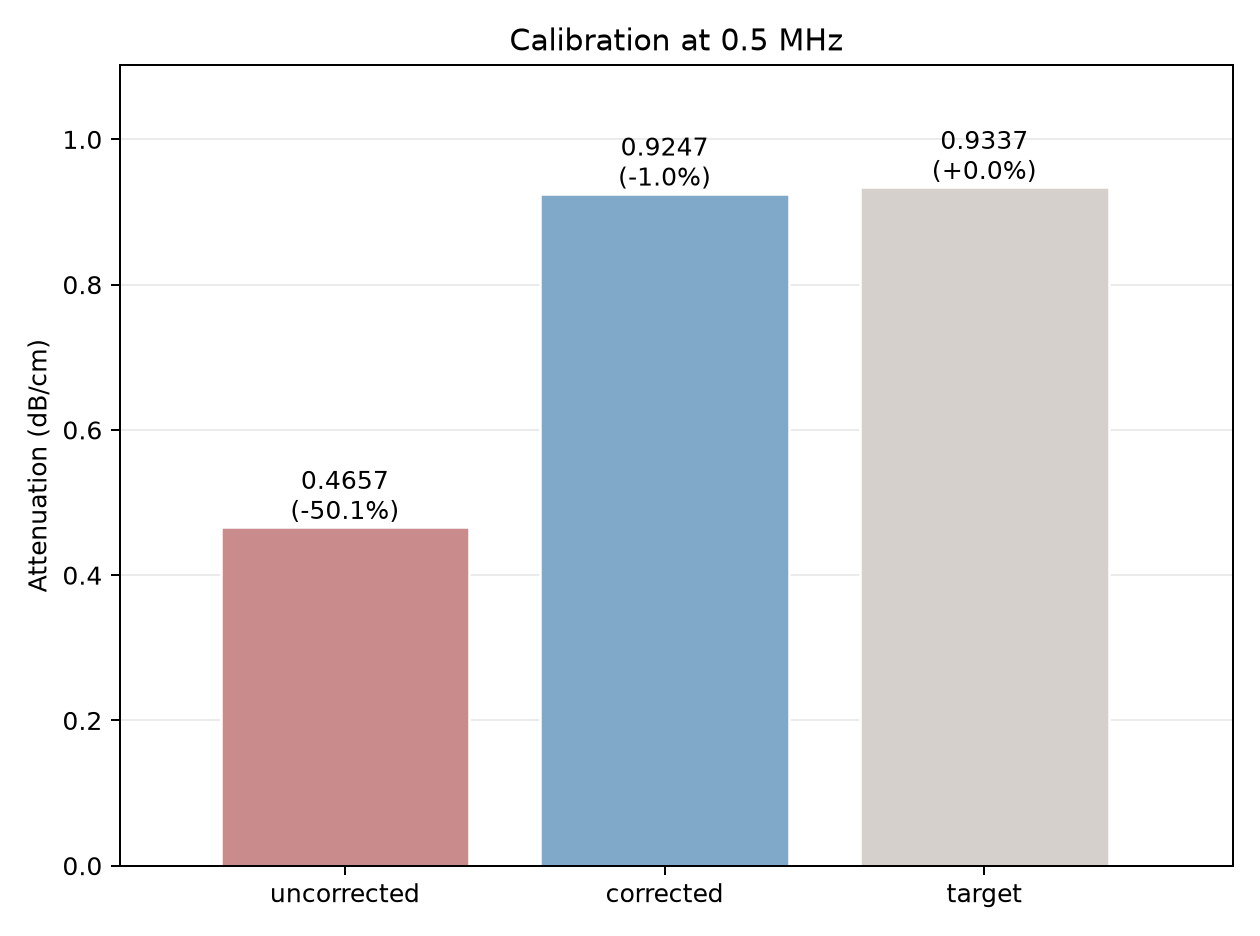
\includegraphics[width=.72\linewidth]{figures/fig1_calibration_bar.png}\caption{Bar chart at 0.5 MHz. Three bars show attenuation in dB/cm: Uncorrected (literature coefficient used directly with y=2), Corrected (coefficient matched to f0 using this project's formula), and Target (the literature y=1 value at f0). Each bar is labeled with its value and percent error versus Target. Matching removes the large calibration bias seen in the Uncorrected bar.}\end{figure}
\begin{figure}[H]\centering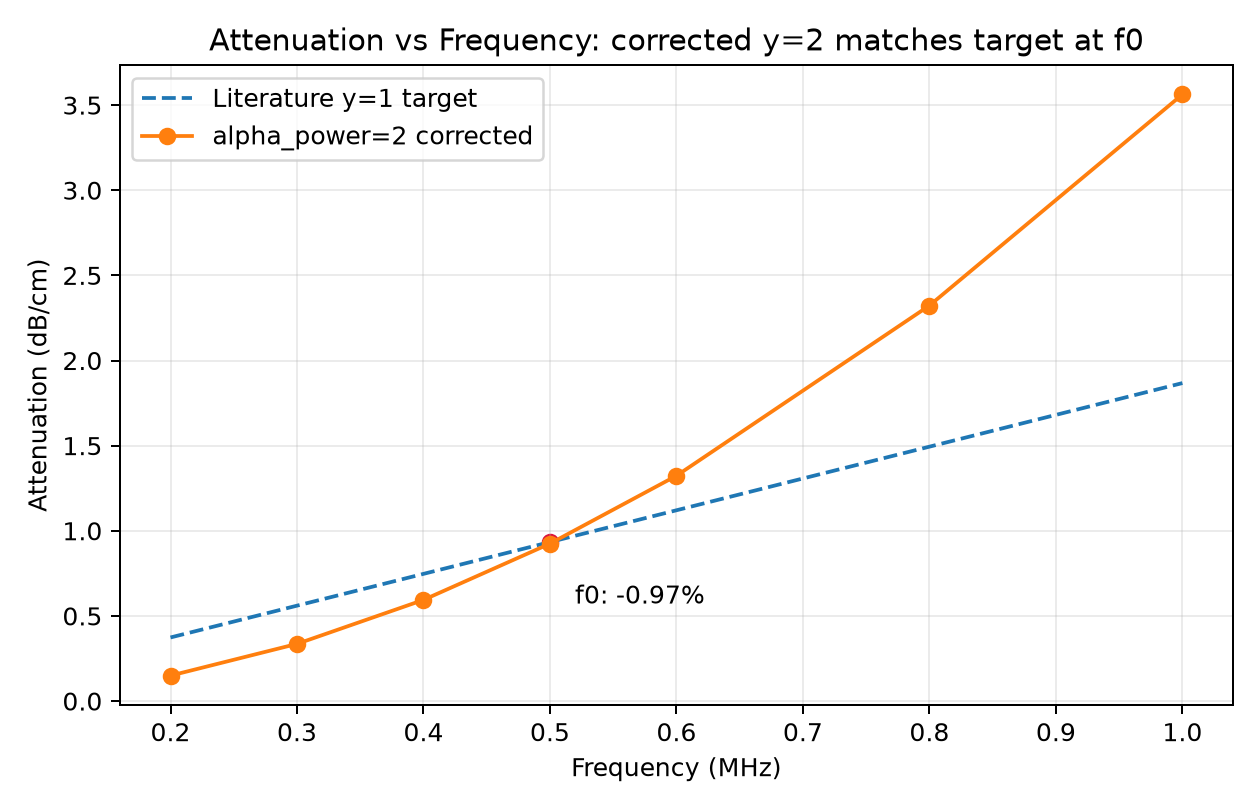
\includegraphics[width=.72\linewidth]{figures/fig2_frequency_sweep.png}\caption{Line chart. X-axis: frequency (MHz), 0.2 to 1.0. Y-axis: attenuation (dB/cm). Dashed line: the literature y=1 target at each frequency. Solid line: the corrected y=2 model's simulated attenuation at each frequency. The two lines meet only at f0=0.5 MHz (marked); away from f0, the y=2 model's attenuation grows faster with frequency than the literature's y=1 line, which is the expected consequence of the exponents differing.}\end{figure}
\begin{figure}[H]\centering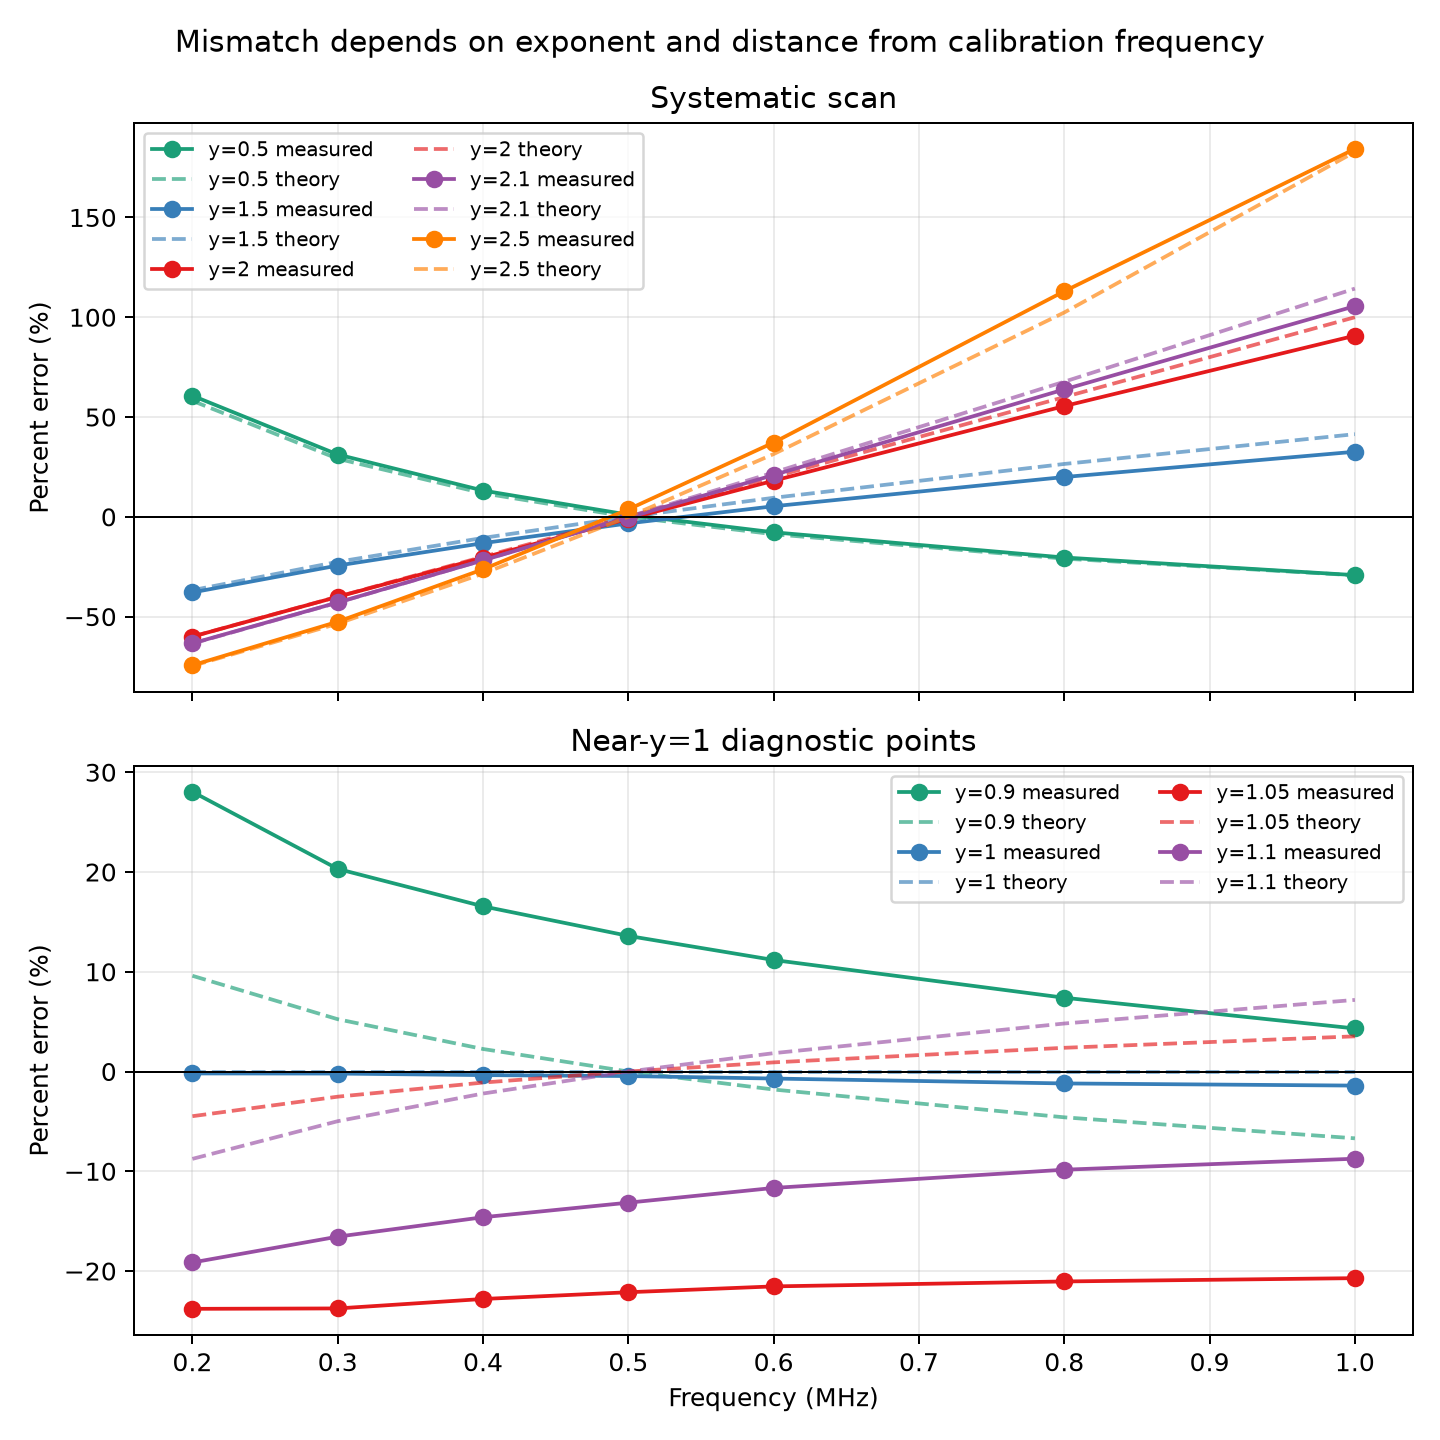
\includegraphics[width=.88\linewidth]{figures/fig3_error_vs_n.png}\caption{Two-panel line chart. X-axis (both panels): frequency (MHz). Y-axis (both panels): percent error versus the literature target. Each exponent y has two lines of the same color: solid = measured (simulated) error, dashed = theoretical error predicted by $(f/f_0)^{y-1}-1$. Top panel: systematic scan points (y=0.5, 1.5, 2, 2.1, 2.5), where measured and theoretical lines closely overlap. Bottom panel: near-y=1 diagnostic points (y=0.9, 1, 1.05, 1.1), where the measured lines for y=1.05 and y=1.1 visibly depart from their theoretical dashed counterparts.}\end{figure}
\begin{figure}[H]\centering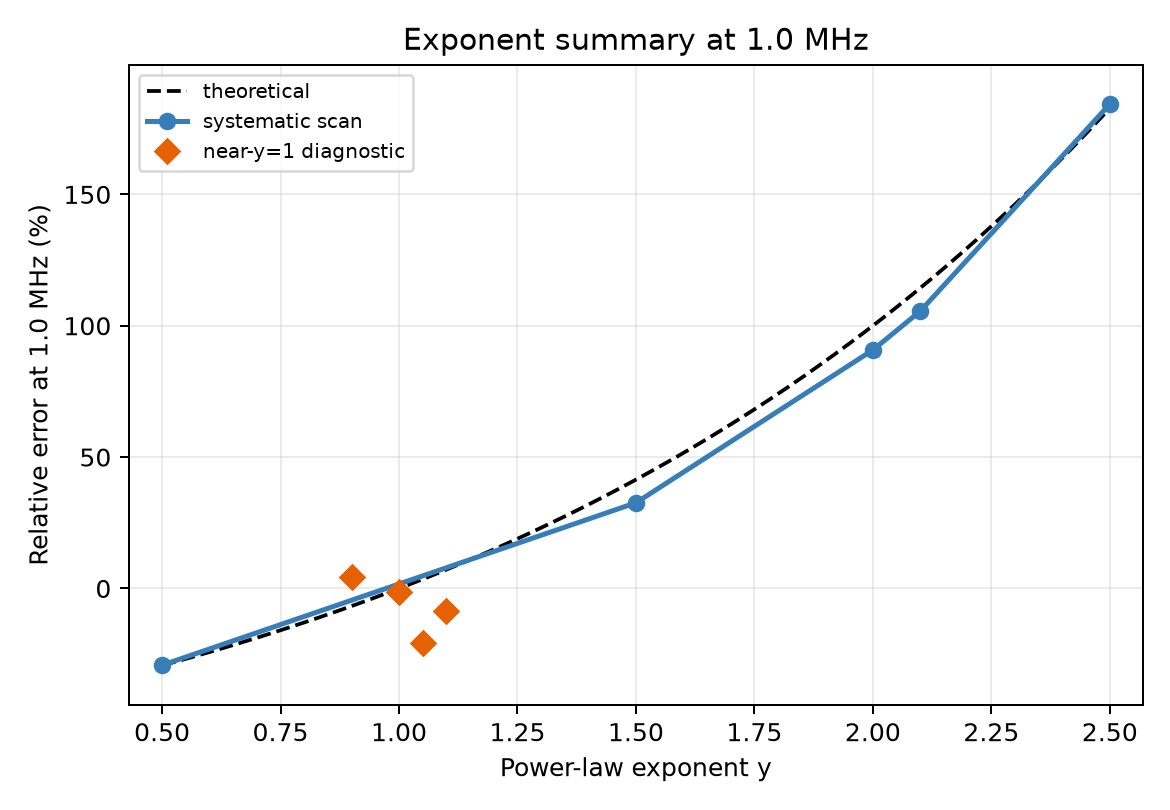
\includegraphics[width=.72\linewidth]{figures/fig4_exponent_summary.png}\caption{Scatter/line chart. X-axis: power-law exponent y, 0.5 to 2.5. Y-axis: relative error (\%) at 1.0 MHz. Black dashed line: ideal theoretical error curve. Blue connected dots: systematic scan points, which closely follow the theoretical curve. Orange diamonds (not connected by a line): near-y=1 diagnostic points, which fall well off the theoretical curve. At 1.0 MHz the theoretical curve is itself far from zero away from y=1, so this panel shows departure from the expected power-law mismatch rather than a $\pm5\%$ calibration band; that band is shown only in Figure~5, where it is evaluated at the calibration frequency.}\end{figure}

The algebraic conversion answers a parameter-transfer question. It does not guarantee that a numerical solver will reproduce the converted attenuation. A high $R^2$ indicates approximately exponential pressure decay over the fitted interval; it does not certify the recovered attenuation coefficient.

\section{Part 2: Near-y=1 sensitivity of peak-pressure attenuation estimates}
k-Wave treats y=1 as a special input. The recommended \texttt{no\_dispersion} mode disables the causal dispersion correction, sacrificing frequency-dependent sound-speed coupling. This is reasonable for a narrowband toneburst but may distort broadband phase. The investigation began with an unexpected 0.2-MHz result; after checking the main boundary-related settings, the same pattern appeared in the exponent sweep. The fine scan reached $+143.11\%$ at y=0.98 and $-41.01\%$ at y=1.02; sampled exponents outside $\pm5\%$ ran from y=0.80 ($+5.48\%$) to y=1.32 ($-5.07\%$), with y=0.78 ($+4.83\%$) and y=1.35 ($-4.71\%$) the adjacent in-band samples. The sharp behavior is consistent with the pole in the $\tan(\pi y/2)$ term of the underlying Treeby--Cox relation. We use that relation as a theoretical interpretation rather than a reconstruction of k-Wave's implementation. The y=1 reference uses \texttt{no\_dispersion} and is excluded from like-for-like comparisons with default-dispersion points.

\subsection*{Control checks}
For the representative y=0.98 case, timestep refinement gave peak-pressure relative errors of 143.11\% (baseline), 143.72\% (dt/2), and 143.79\% (dt/4), with $R^2$ values of 0.9609, 0.9614, and 0.9616. A frequency-domain amplitude fit around the nearest $f_0$ bin gave 210.10\%, 181.49\%, and 181.40\% for the same runs ($R^2=0.5797$, 0.6659, and 0.6663). The controls show estimator dependence; the timestep test did not explain the observed sensitivity. These values are stored in \texttt{results/controls\_y098.json} and are generated by \texttt{src/matlab/run\_controls.m}.
\begin{figure}[H]\centering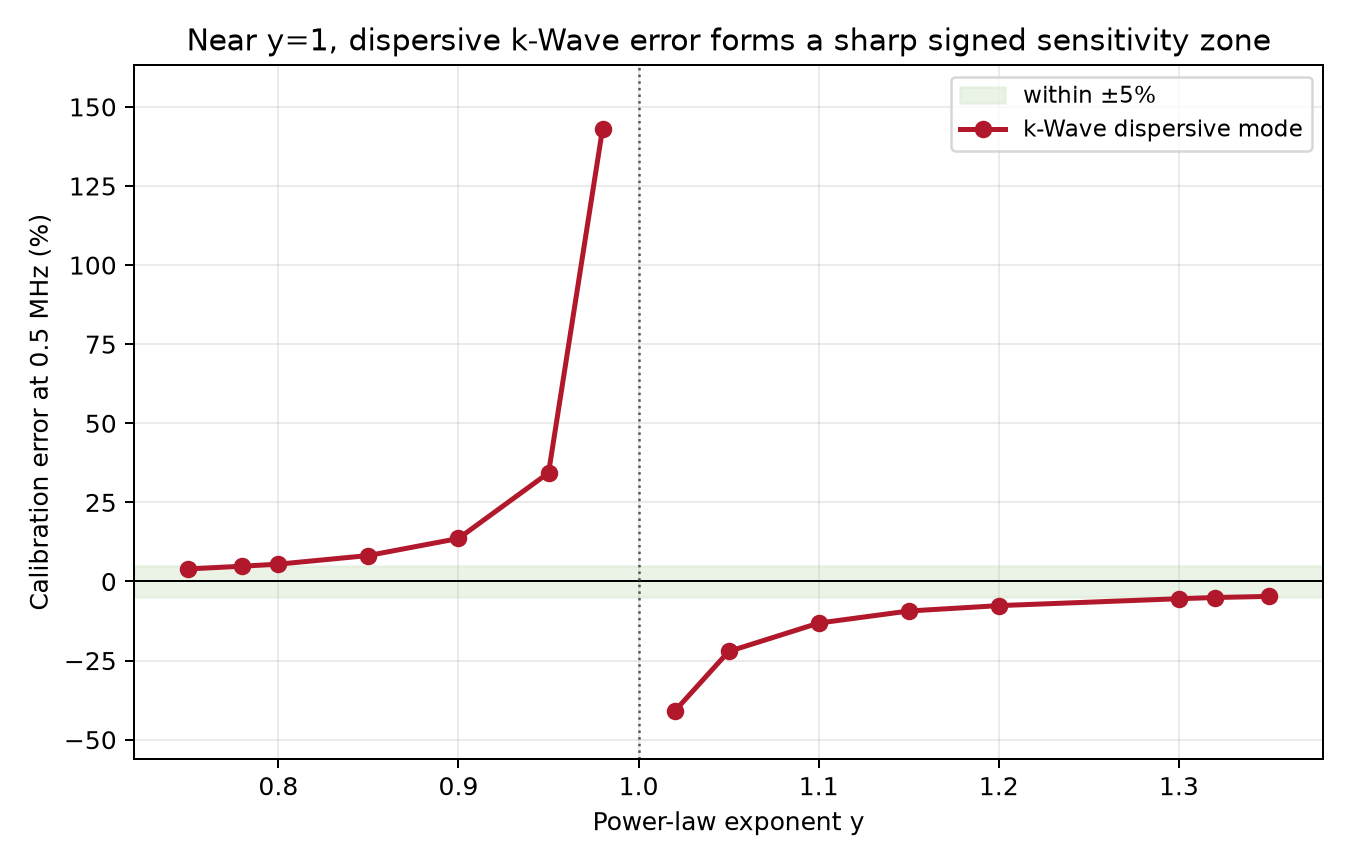
\includegraphics[width=.72\linewidth]{figures/fig5_y1_sensitivity.png}\caption{Line chart, fine scan. X-axis: power-law exponent y, 0.75 to 1.35. Y-axis: calibration error (\%) at 0.5 MHz using default dispersion mode. Shaded green band: within $\pm5\%$ of target. Vertical dotted line: y=1. The error spikes sharply and changes sign on either side of y=1. The curve is drawn as two segments that are deliberately not joined across y=1, because default dispersion has no valid sample there; no interpolation across the singularity is implied.}\end{figure}

\subsection*{Amplitude dependence of the attenuation estimate}
A calibration error is normally read as a fixed multiplicative bias. Near y=1 it is not one. Holding y=1.05 fixed and scaling $\alpha_{\rm coeff}$ by 0.5$\times$, 1$\times$, and 2$\times$ gives measured attenuations of 0.407, 0.727, and 1.189 dB/cm against power-law expectations of 0.451, 0.902, and 1.804 dB/cm, i.e.\ errors of $-9.8\%$, $-19.4\%$, and $-34.1\%$ (Table~\ref{tab:scaling}, \texttt{results/tan\_scaling\_check.json}).

\begin{table}[H]\centering\caption{Scaling of the peak-pressure attenuation estimate with $\alpha_{\rm coeff}$ at y=1.05.}\label{tab:scaling}\begin{tabular}{rrrrr}\toprule Scale & $\alpha_{\rm coeff}$ & Measured (dB/cm) & Power-law expectation (dB/cm) & Error (\%)\\\midrule 0.5$\times$ & 0.9667 & 0.407 & 0.451 & $-9.8$\\ 1$\times$ & 1.9333 & 0.727 & 0.902 & $-19.4$\\ 2$\times$ & 3.8667 & 1.189 & 1.804 & $-34.1$\\\bottomrule\end{tabular}\end{table}

Doubling the coefficient multiplies the fitted attenuation by 1.79$\times$ and then 1.64$\times$, not by 2$\times$. For a wave decaying as $\exp(-\alpha x)$ the fitted slope must be proportional to $\alpha_{\rm coeff}$ whatever the source amplitude, so this compression means the recorded pressure is not decaying exponentially over the fitted interval. Grid refinement does not remove it: at the same exponent, $dx=$ 0.5, 0.25, and 0.125 mm give $-22.12\%$, $-21.86\%$, and $-21.72\%$ (\texttt{results/grid\_resolution\_check.json}), so it is not a discretization artifact.

Two consequences follow. The percentages quoted in this section are conditional on the coefficient used---``$-22.12\%$ at y=1.05'' is the value at $\alpha_{\rm coeff}=1.9333$, not a property of the exponent alone. And the near-y=1 estimate is better read as a distorted peak-pressure observable than as a material attenuation coefficient, which is consistent with the collapse at y=0.99. The same scaling check has not been run at other exponents, so whether this compression is specific to y$\approx$1 or also affects the systematic scan is not established here; that is the most useful follow-up experiment.

\subsection{Fixed-frequency y scans beyond 500 kHz}
Additional scans hold the center frequency at 0.2, 0.3, 0.4, 0.6, 0.8, or 1.0 MHz and vary $y$. New runs add $y=0.98$, 0.99, 1.01, and 1.02 to the existing diagnostic points. Coefficients remain matched at $f_0=0.5$ MHz. Errors use the linear literature target at each tested frequency, so they include the expected power-law mismatch $(f/f_0)^{y-1}-1$ away from $f_0$ as well as deviations of the peak-pressure estimate. Supplementary Figure S1 shows the sampled curves.

\begin{figure}[H]
\centering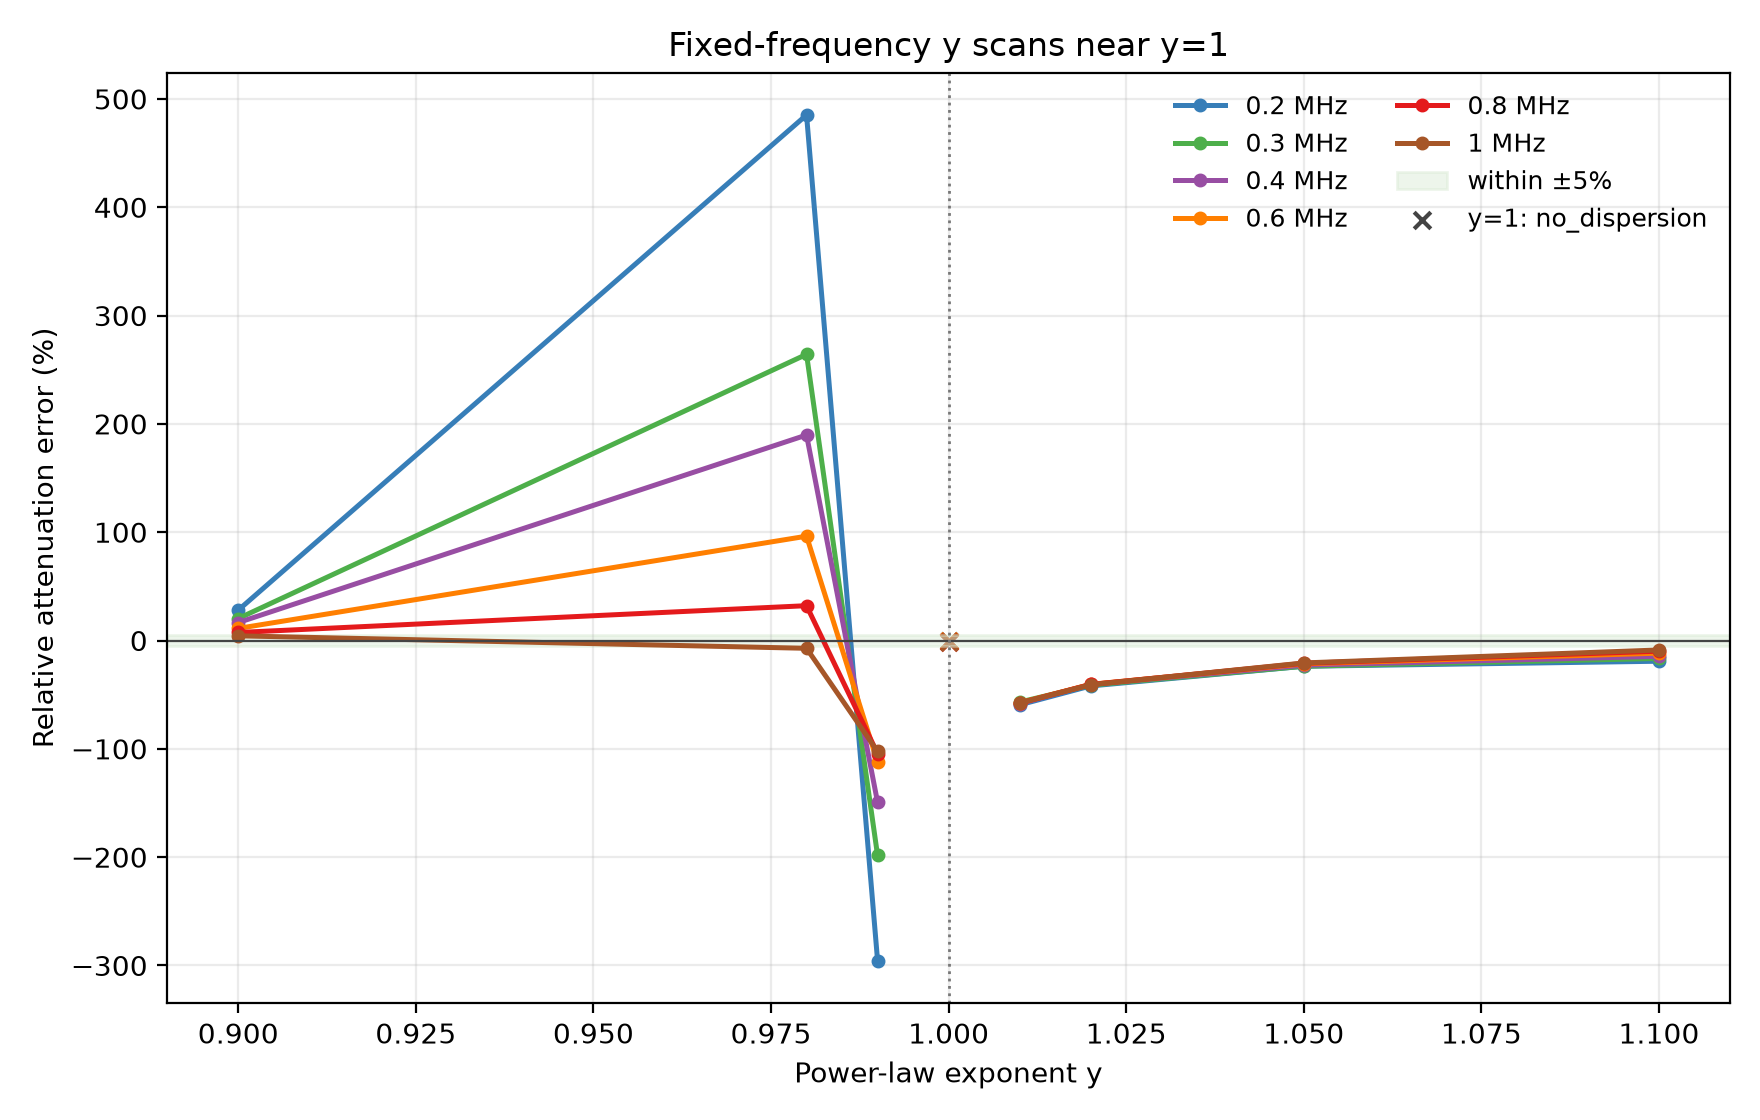
\includegraphics[width=\linewidth]{figures/other_frequencies_error_vs_y.png}
\caption*{Supplementary Figure S1. Fixed-frequency scans versus $y$. Each curve holds frequency fixed. Connected circles use default dispersion, including $y=1.1$; separate crosses at $y=1$ use \texttt{no\_dispersion}. Lines guide the eye between sampled points and do not interpolate across $y=1$. The shaded band marks $\pm5\%$ relative to the linear literature target.}
\end{figure}

The sensitivity extends beyond 500 kHz. At $y=0.98$, errors range from $+485.2\%$ at 0.2 MHz to $-7.2\%$ at 1.0 MHz. At $y=0.99$ the recorded peak pressure collapsed to the $10^{-5}$ Pa level ($1.7\times10^{-5}$ to $7.7\times10^{-5}$ Pa across the six frequencies) and increased with distance (at 0.5 MHz, $7.3\times10^{-5}$ to $9.8\times10^{-5}$ Pa from 26 to 126 mm, $R^2=0.69$--$0.83$), so the fitted slope describes numerical residue rather than a decaying wave; no attenuation estimate is reported for this exponent. At $y=1.01$ and 1.02, errors are approximately $-57\%$ to $-59\%$ and $-41\%$ to $-42\%$, and are nearly flat across the 0.2--1.0 MHz range, where the theoretical power-law mismatch is at most $\pm1.4\%$. A frequency-independent offset of that size is a multiplicative attenuation deficit rather than a mismatch in the frequency exponent.

These exploratory runs use the same configuration as Part 1---in which the source sits inside the PML---with a 90-$\mu$s record and $dx=0.5$ mm. At 0.2 MHz the burst lasts approximately 90 $\mu$s, creating a record-truncation risk. Some near-$y=1$ runs emit a timestep warning. Convergence and estimator controls have not been completed across this matrix; these results do not establish a universal failure interval or a causal explanation. The new JSON files are named \texttt{results/near\_y\_frequency\_y0p98.json}, \texttt{y0p99}, \texttt{y1p01}, and \texttt{y1p02} with the same prefix and extension. The MATLAB driver is \texttt{src/matlab/run\_near\_y\_frequency\_scans.m}.

\section{Relation to existing k-Wave guidance}
k-Wave documentation identifies y=1 as a special case, provides \texttt{no\_dispersion}, and discusses reference-frequency adjustment of $\alpha_{\rm coeff}$. Here, those pieces are tested together under one controlled 1-D setup. This work does not claim novelty for these individual pieces.

Informal k-Wave User Forum discussions provide useful historical context, but they are not peer-reviewed evidence and their version-specific applicability cannot be confirmed here:
\begin{itemize}
\item In a thread dated roughly 2016, one user reported that the \texttt{no\_dispersion} setting made no difference to that user's simulation results (\href{https://www.k-wave.org/forum/topic/attenuation-in-heroginious-medium}{thread}).
\item In a later thread, a user explicitly working with k-Wave 1.2 reported that the C++/CUDA path ignored \texttt{no\_dispersion}, while the MATLAB path used it; the same report described no 3-D difference but a difference in 1-D and suspected an old-version bug (\href{https://www.k-wave.org/forum/topic/attenuation-measurement-in-3d}{thread}). A separate developer reply also stated that the C++/CUDA code did not support \texttt{alpha\_mode} (\href{https://www.k-wave.org/forum/topic/vastly-different-time-of-travel-for-the-same-model-in-3d-and-2d}{thread}).
\item In another discussion, a k-Wave developer explained that \texttt{no\_dispersion} removes one term in the absorption operator: its effect is strongest when the exponent is close to 1 and weaker farther away (\href{https://www.k-wave.org/forum/topic/relationship-between-attenuation-and-wave-velocity}{thread}).
\end{itemize}

The second report concerns k-Wave 1.2. This repository's core 1-D benchmark uses the MATLAB solver. A separate small 3-D backend control found that the tested k-Wave 1.4.1 wrapper/CUDA v1.3 pairing did not apply \texttt{no\_dispersion} and that the CUDA binary rejected exact y=1. The result is stored in \texttt{results/cuda\_y1\_backend\_control\_20260914.json}. In the same 3-D control, y=0.99 under default dispersion produced peak pressures of order $10^{30}$ Pa in both the MATLAB and the CUDA path, and stayed of that order at CFL 0.1, 0.05, and 0.025---a nonphysical field rather than an attenuation value, and one that timestep refinement does not remove. This is a version-specific control, not a claim about every CUDA release. Readers should test \texttt{no\_dispersion} in their own backend, dimensionality, and toolbox version.

Backend portability warning: verifying \texttt{no\_dispersion} in the MATLAB solver does not establish that a GPU/CUDA backend receives or applies the same setting. Before changing an exponent away from a well-tested value, compare default and \texttt{no\_dispersion} outputs on the exact backend used for production.

\section{Part 3: Practical implication and worked example}
The function below is written from scratch to demonstrate this class of error---it isn't lifted from, or meant to represent, any particular codebase.
\begin{verbatim}
% WARNING: illustrative uncorrected mistake pattern; do not copy to production.
function medium = map_hu_to_medium_properties(HUmat)
    psi = max(0, min(1, (1500 - single(HUmat)) / 1500));
    medium.sound_speed = 1483*psi + 2800*(1-psi);
    medium.density = 1000*psi + 1900*(1-psi);
    % WARNING: synthetic HU-to-property mapping; not a validated CT model.
    synthetic_alpha_prefactor_np_per_m_mhz = 21.5 + ...
        (208.9 - 21.5) .* sqrt(psi);
    medium.alpha_coeff = synthetic_alpha_prefactor_np_per_m_mhz * 0.08686;
    medium.alpha_power = 1.1;
    % alpha_mode='no_dispersion' is omitted in the mistake pattern
end
\end{verbatim}
The function above represents a complete synthetic CT-to-medium mapping pattern: sound speed, density, and attenuation vary spatially with \texttt{psi}. If used directly in a heterogeneous simulation, spatial changes in sound speed and density would produce impedance-mismatch reflections, mixing reflection loss with absorption in a transmission-based estimate. The four-row comparison was not produced by running that full heterogeneous mapping. It tests the \texttt{psi=0} pure-cortical-bone limit as a single homogeneous medium, thereby excluding impedance-mismatch reflections from the absorption-calibration check.

For $c=2800$ m/s, $\rho=1900$ kg/m$^3$, $\alpha_{\rm prefactor}=21.5$, y=1.1, and $f_0=0.5$ MHz, the following table reports the simulated comparison.
\begin{table}[H]\centering\caption{Worked-example comparison.}\resizebox{\linewidth}{!}{\begin{tabular}{lrrrr}\toprule Mode & $\alpha_{\rm coeff}$ used & Simulated attenuation (dB/cm) & Error (\%) & $R^2$\\\midrule Default dispersive & 1.867490 & 0.775 & -16.96 & $\approx1$\\ Default dispersive, corrected & 2.001526 & 0.823 & -11.89 & $\approx1$\\ \texttt{no\_dispersion}, uncorrected & 1.867490 & 0.867 & -7.19 & $\approx1$\\ \texttt{no\_dispersion}, corrected & 2.001526 & 0.929 & -0.54 & $\approx1$\\\bottomrule\end{tabular}}
\end{table}
The 0.08686 conversion is correct (1 Np $\approx$ 8.686 dB and 1 m = 100 cm). The -11.89\% value differs from the -13.15\% y=1.1 result in Part 1 because the media differ: Part 1 uses $c=3100$ m/s, $\rho=2200$ kg/m$^3$, whereas this example uses $c=2800$ m/s, $\rho=1900$ kg/m$^3$.
\begin{figure}[H]\centering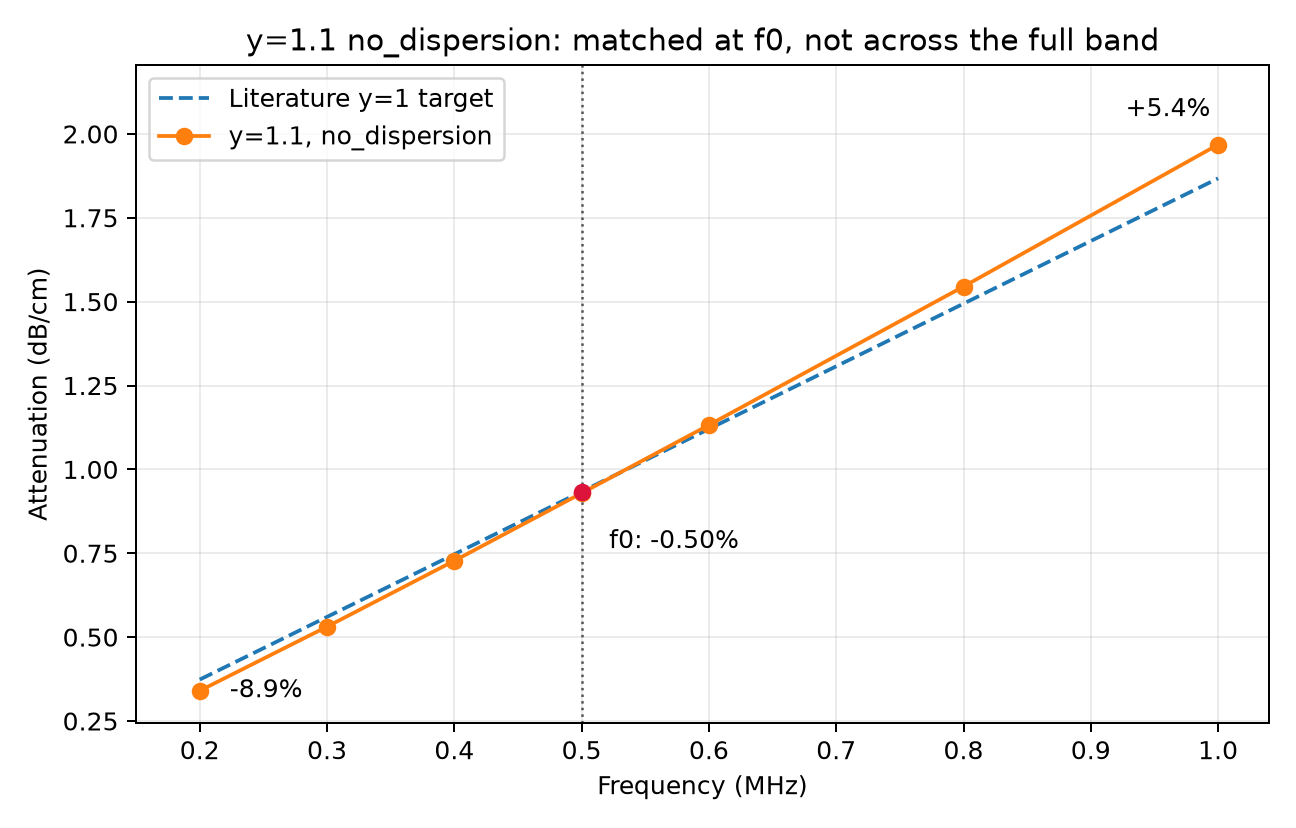
\includegraphics[width=.72\linewidth]{figures/fig6_y11_frequency_scan.png}\caption{Line chart. X-axis: frequency (MHz), 0.2 to 1.0. Y-axis: attenuation (dB/cm). Dashed line: literature y=1 target. Solid line: y=1.1 simulated with no\_dispersion mode, using the matched coefficient. The two lines meet at f0=0.5 MHz but diverge at the band edges, showing that no\_dispersion fixes the calibration point but not the full-band power-law mismatch.}\end{figure}

\section{Conclusion}
Literature attenuation coefficients should be matched to k-Wave's power-law parameterization at the intended operating frequency. This algebraic correction is exact for any exponent k-Wave supports ($0<y\le3$), with y=1 handled as a special case. That correction does not, however, guarantee the numerical attenuation the solver delivers. In default-dispersion mode, exponents near 1---and, by the same $\tan(\pi y/2)$ pole, every odd integer exponent---fail in ways that a percent-error table does not convey: a nearly frequency-independent attenuation deficit ($\approx-58\%$ at y=1.01 over 0.2--1.0 MHz, with a matching $+57\%$ peak-pressure excess in an independent 3-D control), a collapsed wavefield in 1-D at y=0.99, and a divergent one in 3-D at the same exponent. Because the deficit is multiplicative while the collapse is not, the peak-pressure estimate near y=1 should not be read as a material property. In this narrowband 1-D setup, \texttt{no\_dispersion} restores the calibration point, at the cost of frequency-dependent phase coupling.

This study does not determine which attenuation exponent is physically appropriate for skull. It examines how a literature coefficient is transferred into k-Wave for a given exponent, and how the resulting peak-pressure attenuation estimate behaves in the simulation.

\section{Reproduction}
\subsection*{1. Prerequisites}
Install MATLAB R2026a, k-Wave Toolbox 1.4.1, and Python 3.11 or later. MATLAB performs the k-Wave simulation; Python launches MATLAB in batch mode and orchestrates result and figure handling. The driver does not use the Python k-Wave interface or \texttt{matlab.engine}. This project was tested and validated only on MATLAB R2026a. k-Wave 1.4.1 itself may have broader MATLAB version compatibility, but this project has not verified behavior on other MATLAB versions.
\subsection*{2. Configure the environment}
Ensure that \texttt{matlab} is on the system PATH and that the MATLAB scripts can locate k-Wave. From the repository root, install the Python plotting dependencies:
\begin{verbatim}
pip install -r requirements.txt
\end{verbatim}
\subsection*{3. Run the benchmark}
From the repository root, run:
\begin{verbatim}
python src/run_experiments.py
\end{verbatim}
The command calls \texttt{matlab -batch}, writes JSON summaries to \texttt{results/}, and regenerates six figures under \texttt{figures/}. No GPU is required. If MATLAB is not available, the committed JSON summaries are sufficient to redraw the figures with \texttt{python src/run\_experiments.py --plot-only}, which needs only \texttt{numpy} and \texttt{matplotlib} and cannot regenerate the simulations. Not every committed JSON is produced by that driver; \texttt{results/singularity\_scan.json}, \texttt{y11\_no\_dispersion.json}, \texttt{tan\_scaling\_check.json}, and \texttt{grid\_resolution\_check.json} came from earlier one-off runs that are not in the repository, and the README lists the provenance of each file.

Runtime depends on local MATLAB and k-Wave performance and has not been measured systematically for this project.

\subsection*{4. Optional CUDA backend control}
The optional control requires a compatible standalone k-Wave CUDA binary. Configure the toolbox root, binary directory, and binary name through the documented \texttt{TFUS\_KWAVE} environment variables. Then run these scripts from MATLAB:
\begin{itemize}
\item \path{src/matlab/validate_kwave_cuda_y1_nearby.m}
\item \path{src/matlab/validate_kwave_cuda_y1_timestep.m}
\end{itemize}
The committed JSON is a path-sanitized run summary. These controls do not read production data.

\section{Limitations}
\begin{itemize}
\item The attenuation-calibration benchmark is a homogeneous 1-D medium. A separate small homogeneous 3-D control tests backend behavior only; neither experiment represents 3-D skull geometry.
\item The y$\approx$1 sensitivity boundaries (y=0.80--1.32) depend on this grid, PML, and fitting interval. They are not universal constants. The edges are bracketed only by the sampled exponents, so the underlying boundaries lie somewhere in (0.78, 0.80) and (1.32, 1.35).
\item In every 1-D run, including the Part 1 results, the source sits inside the internal PML (grid index 8 with a 20-point PML). This is not standard k-Wave practice and is not ruled out as a contributor to the residual few-percent bias seen even at y=2, or to the non-proportional scaling of the attenuation estimate with $\alpha_{\rm coeff}$. Moving the source into the physical interior and lengthening the domain is a required follow-up.
\item The attenuation estimate is not proportional to $\alpha_{\rm coeff}$ near y=1 (Table~\ref{tab:scaling}), so the percentages quoted in Part 2 are conditional on the coefficient used. The same scaling check has not been run at other exponents.
\item \texttt{no\_dispersion} removes frequency-dependent phase coupling. This has little effect for narrowband or CW sources, since there is no broadband phase content to distort. It can distort phase for short broadband pulses.
\item The $\tan(\pi y/2)$ pole is dimension-independent, but the small 3-D control does not establish its numerical severity for other grids, geometries, or binaries.
\item Attenuation is estimated from peak pressure rather than a fully frequency-resolved spectral attenuation measurement.
\item The current experiments do not completely separate dispersion/model effects from numerical discretization effects.
\item This calibration addresses only the parameter transfer between a literature linear attenuation law and k-Wave's absorption parameters (\texttt{alpha\_coeff} and \texttt{alpha\_power}). In real skull, especially trabecular bone, scattering and longitudinal-to-shear mode conversion can also contribute substantially to acoustic energy loss. Those mechanisms are not represented by \texttt{alpha\_coeff}. Correct absorption calibration therefore does not guarantee agreement with experimentally reported total transmission loss when scattering and mode conversion are present.
\end{itemize}
\textbf{Project structure.} The Python driver orchestrates the core 1-D run, and \path{src/matlab/run_kwave_experiments.m} performs that simulation. Two additional MATLAB scripts provide the isolated CUDA controls. The \texttt{results/} directory stores summaries; \texttt{figures/} stores plots.

\section{Author}
Yue Wang (Yuewang04)

\section{Citation}
Machine-readable metadata is provided in \texttt{CITATION.cff} in the repository root. The archived version is deposited on Zenodo: doi:10.5281/zenodo.23804834 (v1.0.0). The concept DOI 10.5281/zenodo.23804833 resolves to the latest version.

\section*{References}
Aubry et al., \textit{JASA} 152(2), 1003--1019 (2022), doi:10.1121/10.0013426.\\
Treeby and Cox, \textit{JASA} 127(5), 2741--2748 (2010), doi:10.1121/1.3377056.\\
Treeby and Cox, \textit{JASA} 136(4), 1490--1500 (2014), doi:10.1121/1.4894790.\\
Singh et al., \textit{Scientific Reports} 14, 1488 (2024), doi:10.1038/s41598-024-51623-5.\\
Bamber, ``Attenuation and Absorption,'' in \textit{Physical Principles of Medical Ultrasonics}, 2nd ed., Chapter 4 (2004), doi:10.1002/0470093978.ch4.\\
k-Wave documentation, ``The k-Wave Manual / power-law absorption and dispersion,'' \texttt{k-wave.org}.

\section*{Feedback and license}
Questions, corrections, and reproducibility reports are welcome through the repository's GitHub Issues page. This project is licensed under the MIT License; see \texttt{LICENSE}.
\end{document}
